\chapter{Simulation Results}
\label{sec:results}

This section discusses the results we found in this thesis.
The performance of the optimization routine is shown for different settings, that is for different numbers of relays, receiving antennas per user, users, relay placings, and input powers.
Unless otherwise stated, we use the same settings as in Section~\ref{sec:solver}: we look at a two-user system with one receiver antenna and three relays per user, as shown in Figure~\ref{fig:antenna_placing}.
The relays in this system are lossless, meaning that impedance will be pure imaginary.
Additionally, we only consider noise contributions of the circuitry after the LNA, or only downstream noise (c.f. Equation~\eqref{eq:noise_contrib}).
Therefore, because of the unilateral assumption, the noise contribution will be i.i.d. and independent of the matching network or the relays.
Hence, the optimization algorithm only adapts to the signal and the interference.

\section{Introduction of Measures for Comparison}
\label{sec:measures}
In order to rate the results on quality, their performance will be compared to classical interference-eliminating methods such as TDMA.
Additionally, improvements from the uncoupled case will be given as well as theoretical performance limits, in order to see how much the performance can be pushed.
In the following, the rates to which the optimization is compared are introduced.
\begin{figure}[h]
\centering
  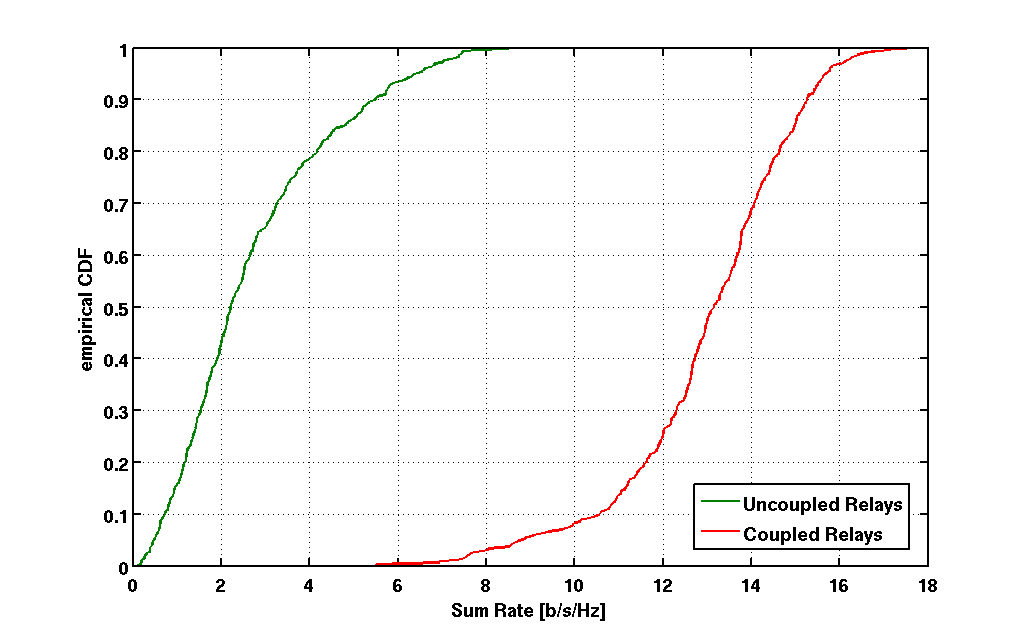
\includegraphics[width=0.85\linewidth]{images/Coupledcomparison.png}
\caption{Comparison of uncoupled relays and optimized coupled relays.}
\label{fig:coupledcomparison}
\end{figure}

\subsection{Uncoupled Relay Rates}
One of the logical comparisons for the use of loaded antennas is the same setting without any coupling among the relays.
Logically, the ``uncoupled relays rate"~----~later sometimes also only ``uncoupled rate"~---~should be smaller than including the relays and adapting their impedances to our needs.
If no higher rate can be achieved, the whole idea of using passive relays would fail.
Hence, the uncoupled relay rate serves as a lower limit which should be achieved.

In Figure~\ref{fig:coupledcomparison}, the green solid line shows the performance if no coupling among the relays and receivers exists.
It is clear that the rates including relay coupling (red solid line) are much larger.
Therefore, this method is suitable for improving achievable rates.


\subsection{TDMA Rates}
In the next step, the optimized rates are compared to the TDMA rates for the equivalent setup.
Therefore, the relays are again assumed to be uncoupled from the receivers and the transmit/receive pairs are assumed to divide time equally among themselves for transmission.
For this calculation the formulas from Equations~\eqref{eq:tdma_achiev_rate} and~\eqref{eq:tdma_achiev_sum_rate} are used.

\begin{figure}[h]
\centering
  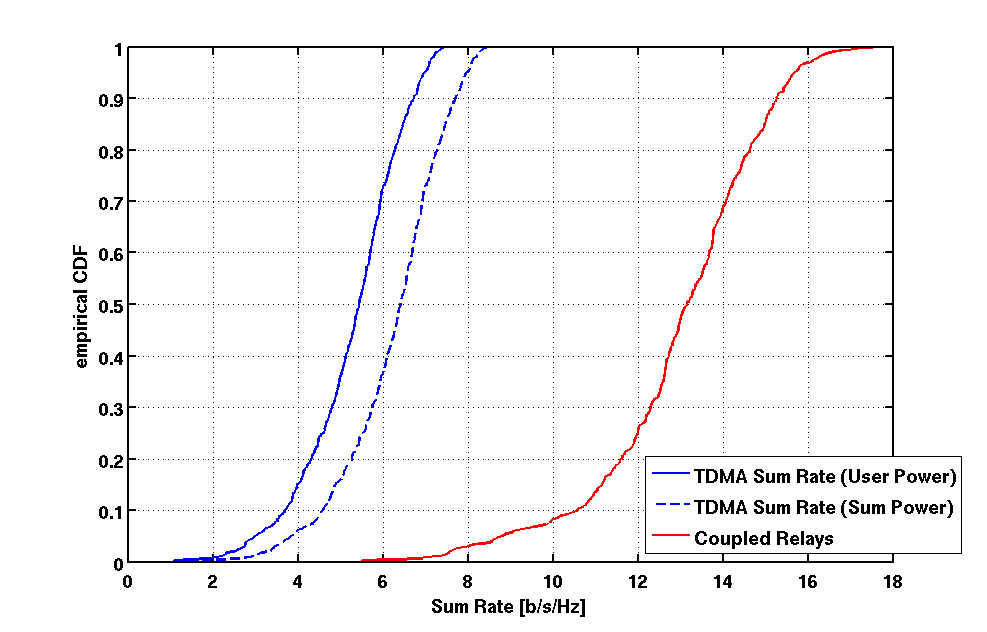
\includegraphics[width=0.9\linewidth]{images/TDMAcomparison.png}
\caption{Comparison of the TDMA rate and optimized coupled relays.}
\label{fig:TDMAcomparison}
\end{figure}

In Figure~\ref{fig:TDMAcomparison}, the blue solid line shows the performance if TDMA is applied under the user-power constraint (i.e. the limit of the transmit power is given for each user and is therefore the same for each user as in the coupled relay case) and the relays are uncoupled from the receivers.
The blue dashed line shows the performance of TDMA under the sum power constraint (i.e. the limit of the transmit power is given by the total transmit power and therefore the power per user in TDMA is $N_\text{User}$ times the power per user in the coupled relay case~----~here two times).
As before, the rates including relay coupling (red solid line) are much larger than those without any coupling and TDMA.
Of course, this comparison is more dependent on the choice of the settings~----~especially the choice of the number of transmit-receive pairs~----~and we will see different behaviors in the following sections. 

\subsection{Noise-free Rates}
\label{sec:sir}
As we are addressing the problem of interference, a good measure is the noise-free rate (SIR-rate).
It is calculated similarly to the SINR-rate, however it only considers the interference and not the noise (c.f. Equation~\eqref{eq:sir_rate}).
As written in the previous chapters, in high-SNR regimes, the interference is the main diminishing factor for achievable rates (c.f. Section~\ref{sec:rates}), and the SIR-rates will give an indicator of how well the relays and matching network are optimized.
Example curves of the SIR-rates (blue dashed lines) can be seen in Figures~\ref{fig:relcomp_1}~to~\ref{fig:relcomp_3}.

\subsection{Relays as Full-Cooperation Receivers - Limit}
\label{sec:fullrx_limit}
The remaining two function against which the rates after our optimization algorithms are compared give limits on how good the method of loaded antennas can potentially be.
The first approach is to consider relays as full-cooperation receivers, which are widely spread.
Hence they experience no coupling among themselves and are spatially uncorrelated.
The number of observations the receiver has on the incoming signals is increased to $N_\text{Rx} + N_\text{Relays}$.
As we choose the number of relays to be larger than the number of interferers in most cases, this method will lead to an interference-free connection.

The performance of the full-cooperation relays can be seen in Figure~\ref{fig:limcomparison} (black solid curve).
At the median it is almost $2 \left[\text{b/s/Hz}\right]$ higher than the optimized rate of the passive coupled relays.
For the best 10\% of cases, this is reduced to $1 \left[\text{b/s/Hz}\right]$ or lower;
for the worst 10\% of cases, it lies between  $2.5 \left[\text{b/s/Hz}\right]$ and $4.7 \left[\text{b/s/Hz}\right]$.


\subsection{Multiport Matching - Limit}
\label{sec:mp_limit}
It has been shown that the multiport matching is the optimal setting for a matching network, without considering any relays~\cite{Nossek}.
For our comparison with the coupled relays, the relays are assumed to be full-cooperating receiver antennas.
\begin{figure}[h]
\centering
  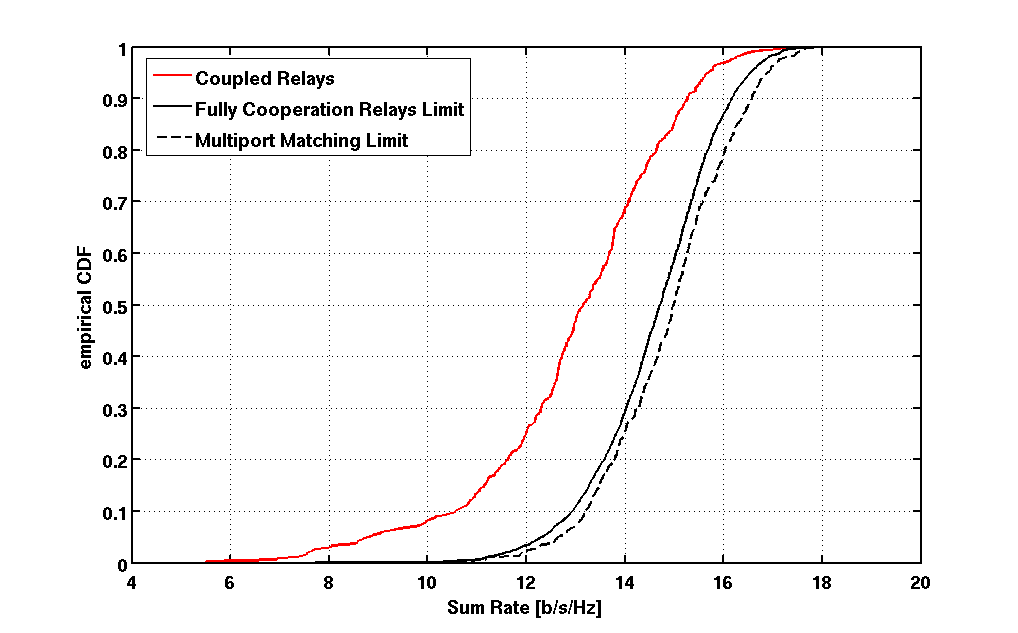
\includegraphics[width=0.9\linewidth]{images/Limitcomparison.png}
\caption{Comparison of the full cooperation relay rates, multiport matching rate and optimized coupled relays rate.}
\label{fig:limcomparison}
\end{figure}
However, the placement of the relays remains the same, so no widely spread receivers are assumed.
The number of observations for each receiver, is $N_\text{Rx} + N_\text{Relays}$ again.
Hence, it can be expected that the new rate is higher than the optimized coupled relays rate.
In Figure~\ref{fig:limcomparison} and the following, this limit is shown by the black dashed line.

\section{Relay Placing}
\label{sec:relay_placing}
Before analyzing the solver with different settings, we discuss the placement of relays around a receiver in more detail.
Figure~\ref{fig:cloud} shows the criteria by which the relays are placed.
\begin{figure}[h]
\centering
  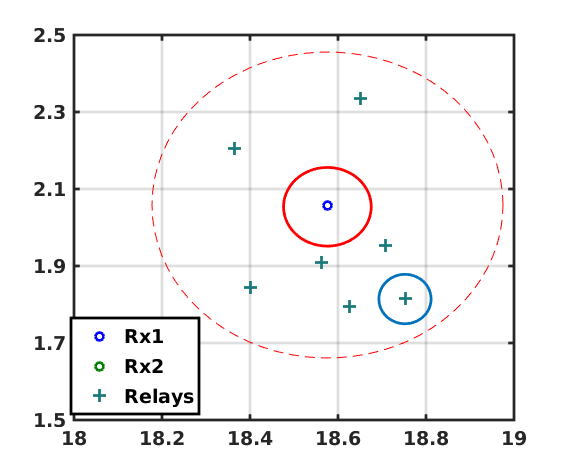
\includegraphics[width=0.6\linewidth]{images/cloud.png}
\caption{Placing the relays around a receiver uniformly distributed on a disc.}
\label{fig:cloud}
\end{figure}
The red solid circle with radius $d_\text{z}$ denotes a zone around the receiver in which no relays must be placed.
The red dashed line shows the maximum distance at which the relays may be placed away from the receiver. 
Within those two lines, the relays are thrown uniformly at random.
The blue circle with radius $d_\text{Relay}$ around the relay at the right bottom denotes a zone in which no other relay may be placed, or the minimum distance between each relay.
If there is a violation of the relay distances, all relays are thrown again.
\begin{figure}[h]
\centering
  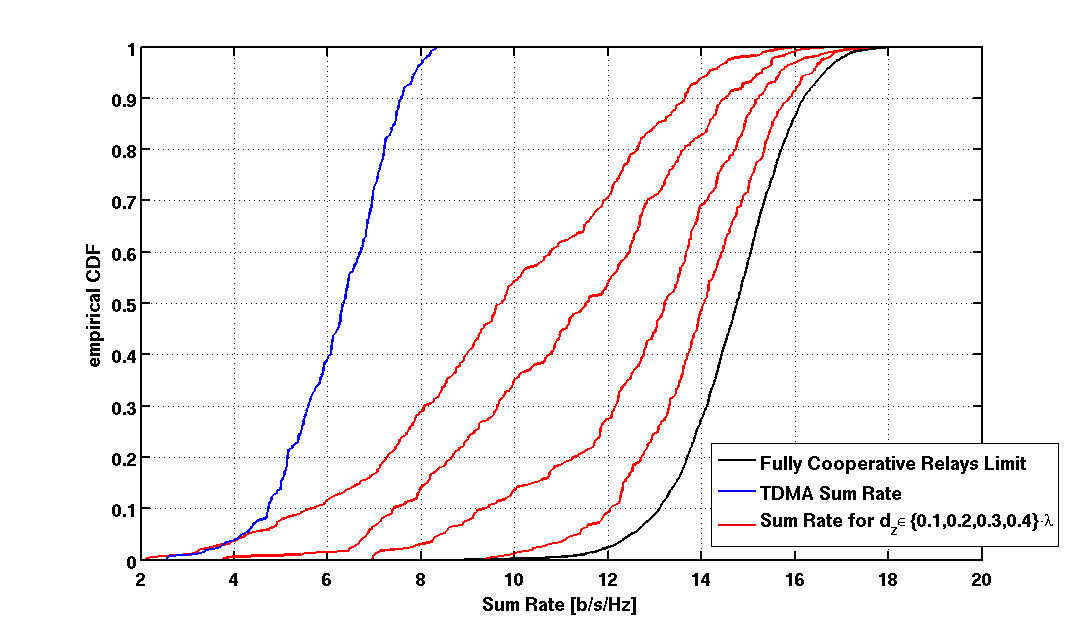
\includegraphics[width=0.8\linewidth]{images/Dzcomparison.png}
\caption{Optimized Sum Rates for different minimum distances between receiver and relays ($d_\text{z}\in\{0.1,0.2,0.3,0.4\}$ from right to left).}
\label{fig:dz_comparison}
\end{figure}

The minimum receiver distance and the minimum relay distance might differ, but unless otherwise specified they are both assumed to be $0.1\lambda$.
With a smaller choice of maximum distance, the relays can be placed more densely.
When the maximum distance is set equal the minimum distance, the relays will be placed along the perimeter of a circle around the receiver.

Figure~\ref{fig:dz_comparison} shows the performance of the optimized sum rate for $d_\text{z}\in\{0.1,0.2,0.3,0.4\}\cdot\lambda$ (red curves from right to left) and the same maximum distance.
For all of the curves, the relays had the same minimum spacing of $d_\text{Relay}=0.1\cdot\lambda$.
Obviously a higher rate can be achieved when the relays are closer to the receiver and thus the coupling is stronger.
Even with a minimum distance of 0.4$\lambda$, the achievable rate is higher than the the TDMA rate (blue solid curve) under the sum power constraint.

\section{Low SNR performance}
\label{sec:low_snr}

First, we analyze the optimization algorithm at different SNR levels.
Later we will only look at a high SNR level, as our aim is to minimize the interference.
As we assume only downstream noise, the optimization algorithm can only change the signal and interference covariance matrices.
\begin{figure}[h]
\centering
  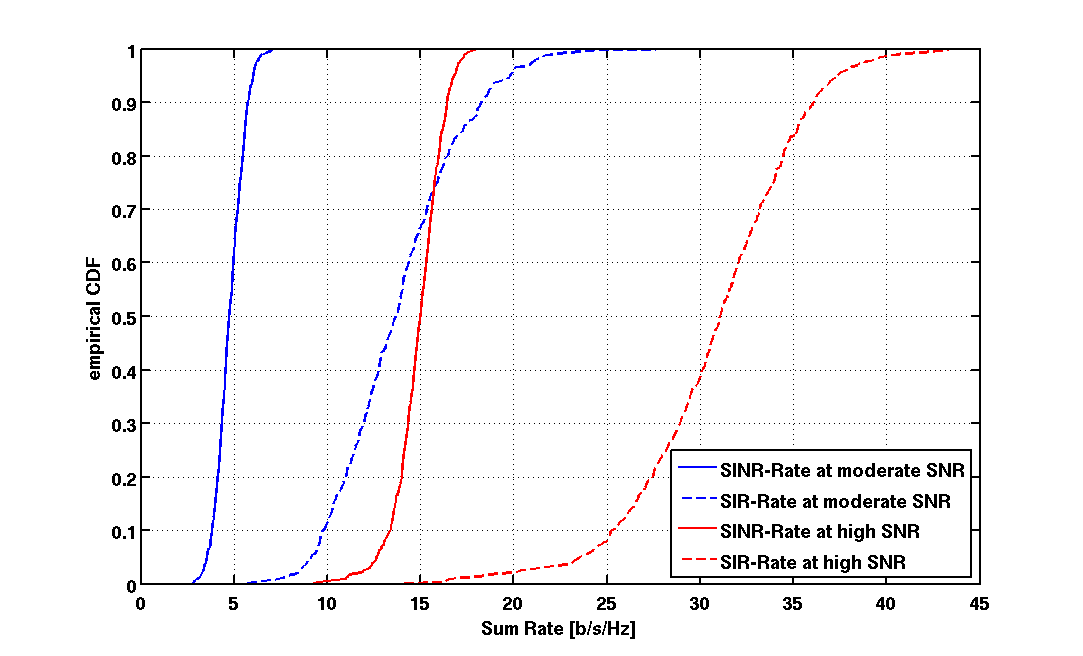
\includegraphics[width=0.9\linewidth]{images/Comparison_modvshighSNR.png}
\caption{Comparison of the optimization algorithm at a moderate and high SNR level and the comparison to the noise free (SIR) rates.}
\label{fig:snrcomparison}
\end{figure}

Figure~\ref{fig:snrcomparison} shows the SINR- and SIR- rates at a moderate SNR level (blue curves) and at a high SNR level (red curves).
As the achievable rate at a moderate SNR level (blue solid line) is less interference-driven and more noise-limited, the resulting SIR-rate (blue dashed curve) is also lower than the SIR-rate of the optimized achievable rate at a high SNR region (red dashed line).

This shows that, for the moderate SNR level, the optimization algorithm matches the values of the relays and the matching network in order to first amplify the signal and only second reduce the interference.
For two users (as is here the case) the interference is increased at the same rate as the signal power (from moderate SNR to high SNR).
If the optimization would have allowed the same reduction of the interference at the moderate SNR level, the SIR rates would have become equivalent.

\section{Number of Relays for Eliminating Interference}
\label{sec:interf_fix}
In the following, the number of relays required for an interference-free connection is determined.
For the following plots, the number of receivers is set to one ($N_{R} = N_{R_x} = 1$) in order to increase the performance of the solver (c.f. Section~\ref{sec:stepwise}).

In the following sections the term ``\textit{interference-free}" will be used.
This term indicates only reduced interference.
Full interference elimination~---~as in a MIMO system with more receiver antennas than interferers~---~will not be reached.
However, when the term is used the interference will be so low that the effect of noise will be an equivalent or even stronger diminishing factor.

\subsection{One Interferer}
\label{sec:1interf}
To eliminate interference with two transmitters, two observations are normally required.
Figure~\ref{fig:relcomp_1} shows the performance of a transmit/receiver pair with one interferer and $N_\text{Rel}\in\{1,2,3\}$ (red curves from left to right).
\begin{figure}[h]
\centering
  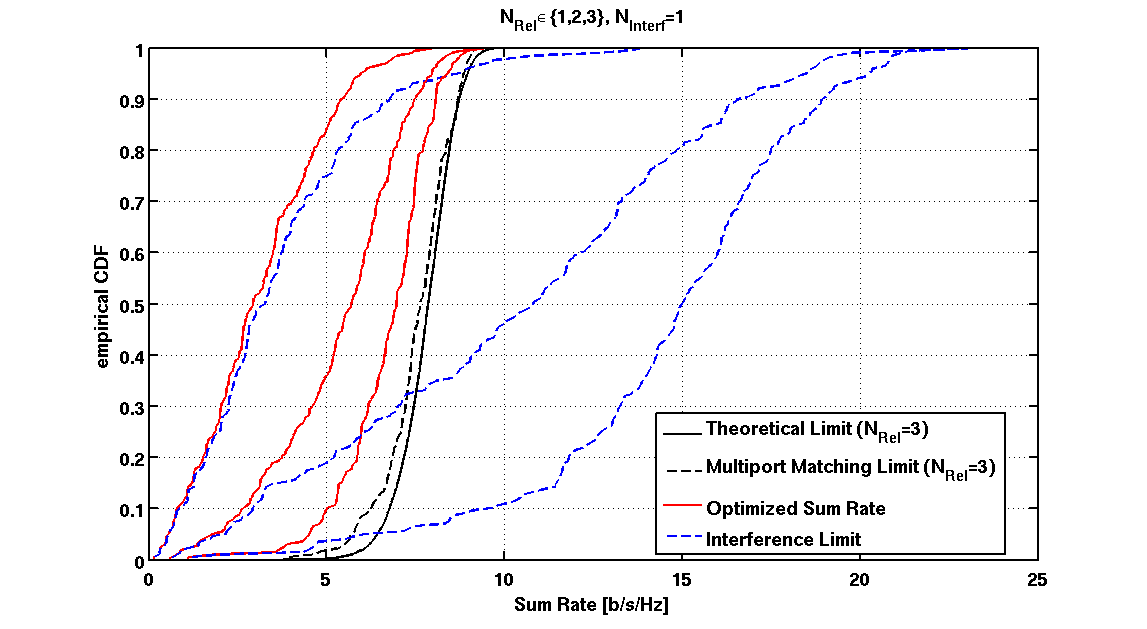
\includegraphics[width=0.9\linewidth]{images/Relcomparison_1interferer.png}
\caption{User rates for one interferer and one receiver with  $N_\text{Rel}\in\{1,2,3\}$ (red and blue curves from left to right) and their theoretical limits (black curves).}
\label{fig:relcomp_1}
\end{figure}
It is clear to see, that higher the numbers of relays, yield better performance in the optimized system.
The blue dashed lines show the rates considering only the SI-ratio (c.f. Equation~\eqref{eq:sir_rate}).
The use of only one relay leads to an interference-free connection for only 10\% of cases.
Increasing the number of relays to two leads to an interference-free connection of almost 80\% of cases.
Achieving a noise-limited connection requires at least three relays per receiver in almost all cases.

\subsection{Two Interferers}
\label{sec:2interf}
To eliminate interference with three transmitters, three observations are normally required.
Figure~\ref{fig:relcomp_2} shows the performance of a transmit/receiver pair with two interferers and $N_\text{Rel}\in\{2,3,4,5\}$ (red curves from left to right).
As before, the blue dashed lines show the rates considering only the SI-ratio.
\begin{figure}[h]
\centering
  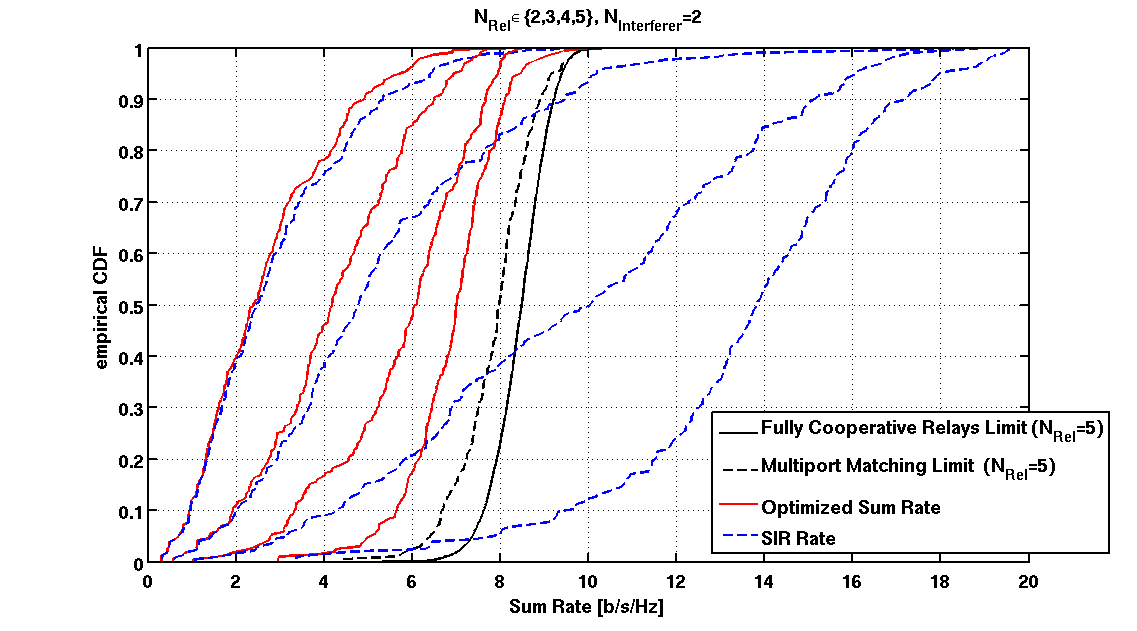
\includegraphics[width=0.9\linewidth]{images/Relcomparison_2interferer.png}
\caption{User rates for two interferers and one receiver with  $N_\text{Rel}\in\{2,3,4,5\}$ (red and blue curves from left to right) and their theoretical limits (black curves).}
\label{fig:relcomp_2}
\end{figure}

We see that, for two relays per user, the interference-limited rate behaves almost the same as the optimized achievable user rate.
For three relays per user, some cases lead to an interference-free connection.
Only in the case of five relays per user can over 90\% of cases be driven into a low-interference state.

\subsection{Three Interferers}
\label{sec:3interf}
To eliminate interference with four transmitters, four observations are normally required.
Figure~\ref{fig:relcomp_3} shows the performance of a transmit/receiver pair with three interferers and $N_\text{Rel}\in\{4,5,6,7\}$ (red and blue dashed curves from left to right).
\begin{figure}[h]
\centering
  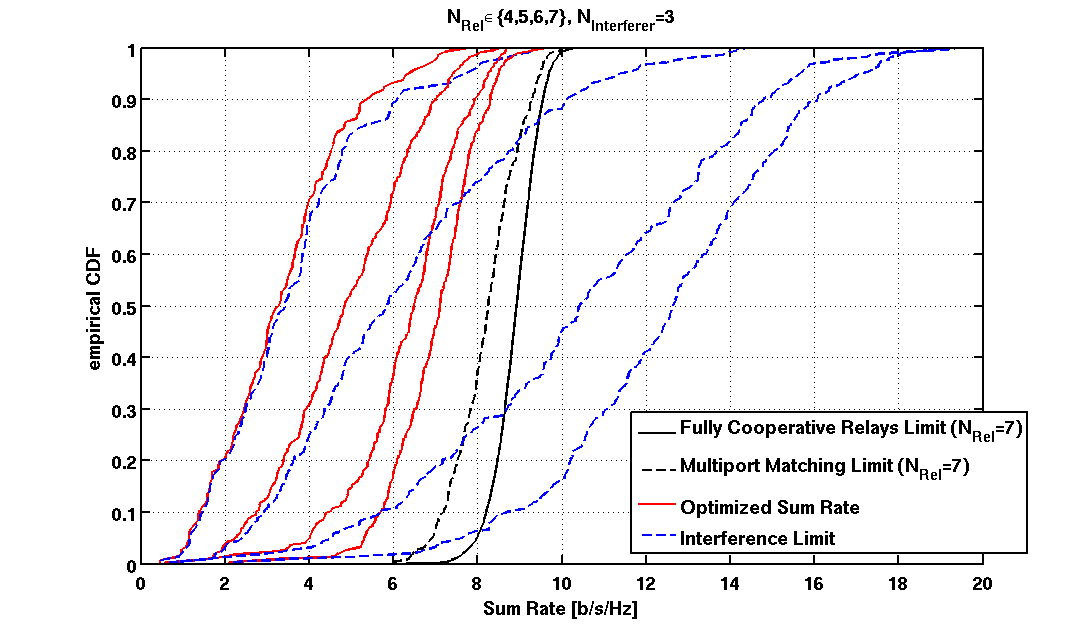
\includegraphics[width=0.9\linewidth]{images/Relcomparison_3interferer.png}
\caption{User rates for three interferer sand one receiver with $N_\text{Rel}\in\{4,5,6,7\}$ (red and blue curves from left to right) and their theoretical limits (black curves).}
\label{fig:relcomp_3}
\end{figure}

We see that, for four relays per user, the interference-limited rate behaves almost the same as the optimized achievable user rate.
For five and six relays per user, some cases lead to an interference-free connection.
For seven relays per user, over 90\% of cases can be driven into an low-interference state.

Comparing this to the previous results with one and two interferers, we can see that  the number of relays required to eliminate interference does not grow linearly as with the use of fully cooperating receivers.
It appears that it requires at least twice the number of interferers ($N_\text{Rel} > N_\text{Interferer}\cdot2$) per user to overcome the interference.

\subsection{Cooperative versus Non-cooperative Receive Antennas}
\label{sec:rel_rx_comp}
In the following, we analyze what happens if the number of relays plus receiver antennas is kept constant.
First, we analyze the case of one receive/transmit pair and three interferers, as this decreases the size of the problem by a factor of four.
Behaviors like those in Section~\ref{sec:stepwise} are therefore less likely to occur.
\begin{figure}[h]
\centering
  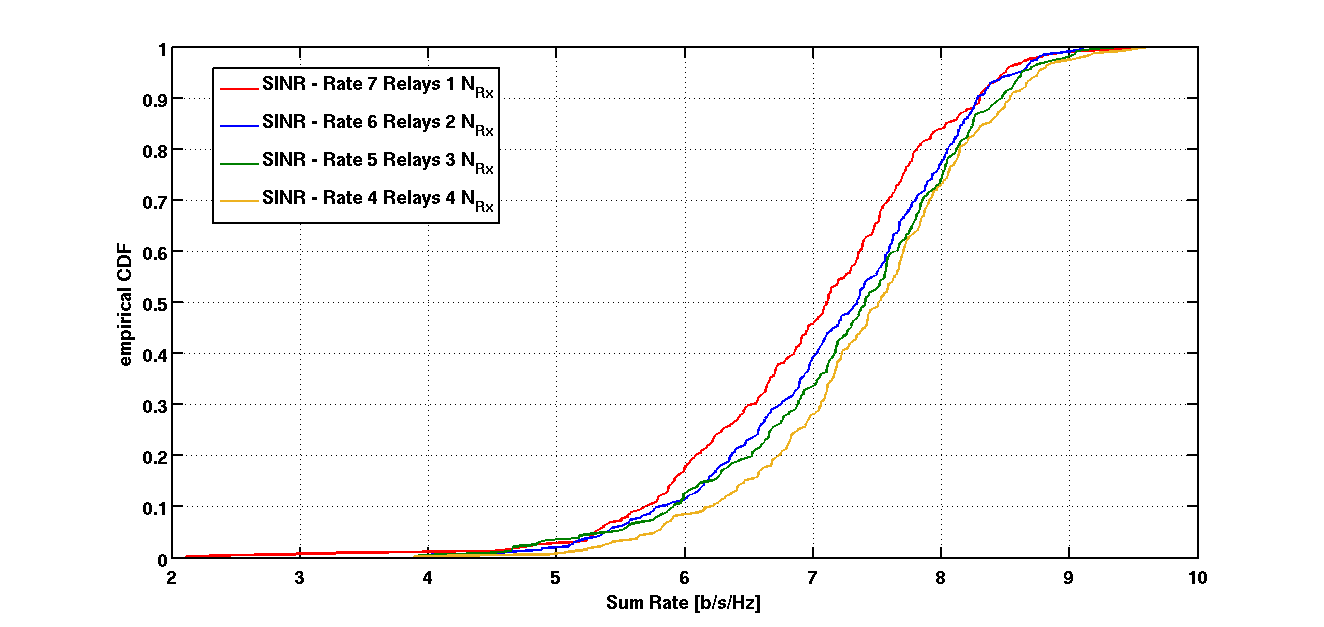
\includegraphics[width=\linewidth]{images/ConstNrelNrx8comparison_1Rx_onlySINR.png}
\caption{Comparison of constant $N_\text{Rel} + N_{\text{Rx}} = 8$, with $N_\text{Rel}\in\{4,5,6,7\}$ and $N_{\text{Rx}}\in\{1,2,3,4\}$ from left to right.}
\label{fig:1user_const}
\end{figure}
%\subsection{Constant Number of Receivers and Relays}
%\label{sec:1user_const}

Figure~\ref{fig:1user_const} shows the performance with three interferers and one transmit/receive pair.
Obviously in the case where four receiver antennas are used (yellow curve), the interference can be fully zero-forced and therefore it also shows the highest rate.
However the performance is only $0.5 \left[\text{b/s/Hz}\right]$ smaller if seven relays and only one receive antenna are used (red curve)~---~even less for the values in between (blue and green curves).
This shows that, with one additional observation and one fewer relay, the rate cannot be improved significantly.
\begin{figure}[h]
\centering
  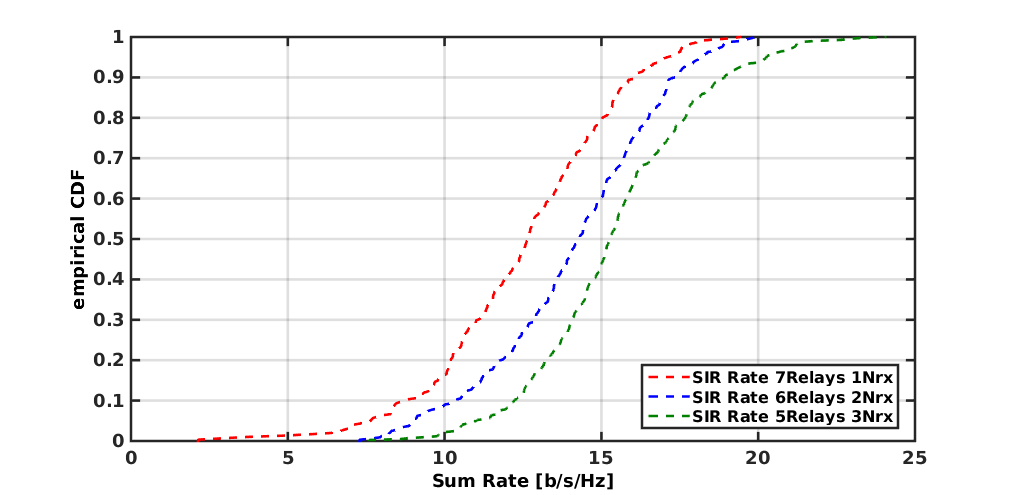
\includegraphics[width=0.9\linewidth]{images/ConstNrelNrx8comparison_1Rx_onlySIR.png}
\caption{Comparison of constant $N_\text{Rel} + N_{\text{Rx}} = 8$, with $N_\text{Rel}\in\{4,5,6,7\}$ and $N_{\text{Rx}}\in\{1,2,3,4\}$ from left to right, showing only noise free rates.}
\label{fig:1user_const_SIR}
\end{figure}
Therefore we can stick with a system that uses one receiver antenna and multiple relays, and can expect to perform similarly to a MIMO system with a sufficiently large number of receiver antennas to zero-force any interference.

Figure~\ref{fig:1user_const_SIR} shows the noise free, hence interference-limited rates for a constant number of relays and receivers.
The SIR-rate for the receiver with four antennas is neglected, as the interference can be fully eliminated.
Again, it can be seen, that the larger the number of receive antennas, the better the interference can be reduced.
However, the differences are~---~as mentioned above~---~small.
Therefore we can conclude, that a system can almost perform the same by increasing the numbers of relays, as it would increasing the number of receive antennas.
Additionally, the problem complexity is kept smaller by using relays, as one receive antenna adds three variable by the matching network, but one relay only adds one variable for its load.

\section{Four User System}
In the previous sections, the requirements for a system with three interferers were given.
Therefore in the following sections a full-four user system will be analyzed to determine whether the conclusions drawn from the previous sections are correct.

\subsection{Prediction for four Users}
\label{sec:const_prediction}

Using the results shown in the previous section, the performance of a four-user system can now be predicted.
A simulation of a four-user system with widely spread receivers should lead to the same results as would summing up the previous curves four times.
\begin{figure}[h]
\centering
  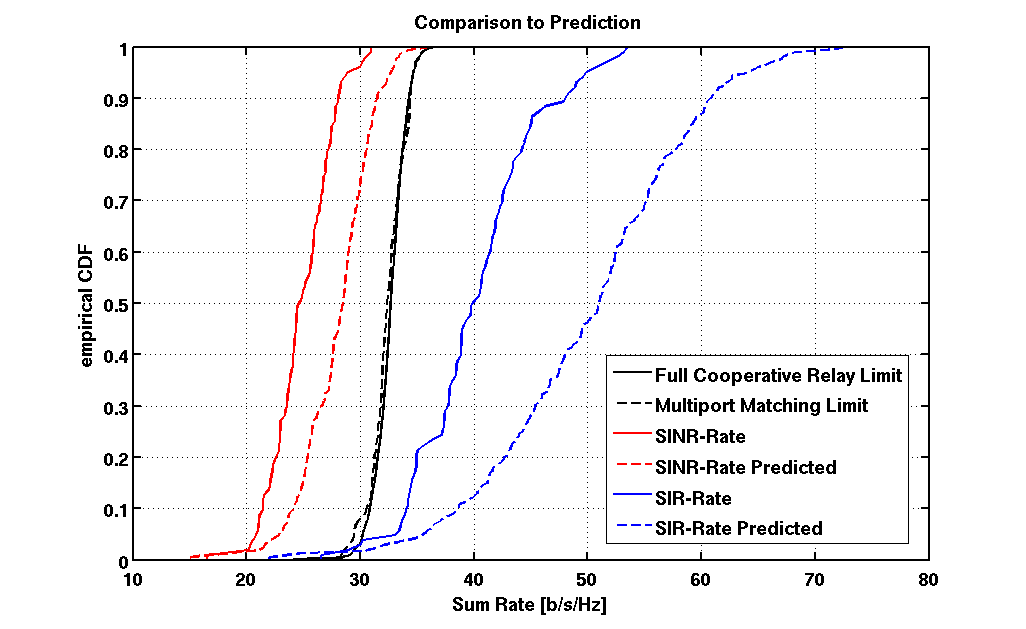
\includegraphics[width=\linewidth]{images/4user_inklpred.png}
\caption{Plot of the 4 User System, with the predicted performance.}
\label{fig:4user_pred}
\end{figure}

Figure~\ref{fig:4user_pred} shows predicted performances (dashed lines) compared to simulated performances (solid lines).
The rates of the simulated realizations are lower than the predicted behavior.
For the simulation, the receivers were not placed widely apart, which is one reason for the lower rates as the non optimized coupling among receivers diminishes the performance.
The second reason is, as mentioned above, the lower performance of the optimization algorithm with a larger problem.
Still, we can conclude that the optimal solution must be between the solid and the dashed curves.

Additionally, the black curves give the theoretical limits of the sum rates.
Because the predicted performance does not outperforme the theoretical limits, it follows that the optimal solution lies near the predicted performance.


\subsection{Full Four-User System Performance}
\label{sec:4user_const}

Finally we analyze the relay and matching network optimization of a four-user system.
Two typical realizations and antenna placings can be seen in Figure~\ref{fig:4user_placing}.
The achievable rates after optimization are analyzed in the following for such and other placings.
\begin{figure}[h]
\centering
  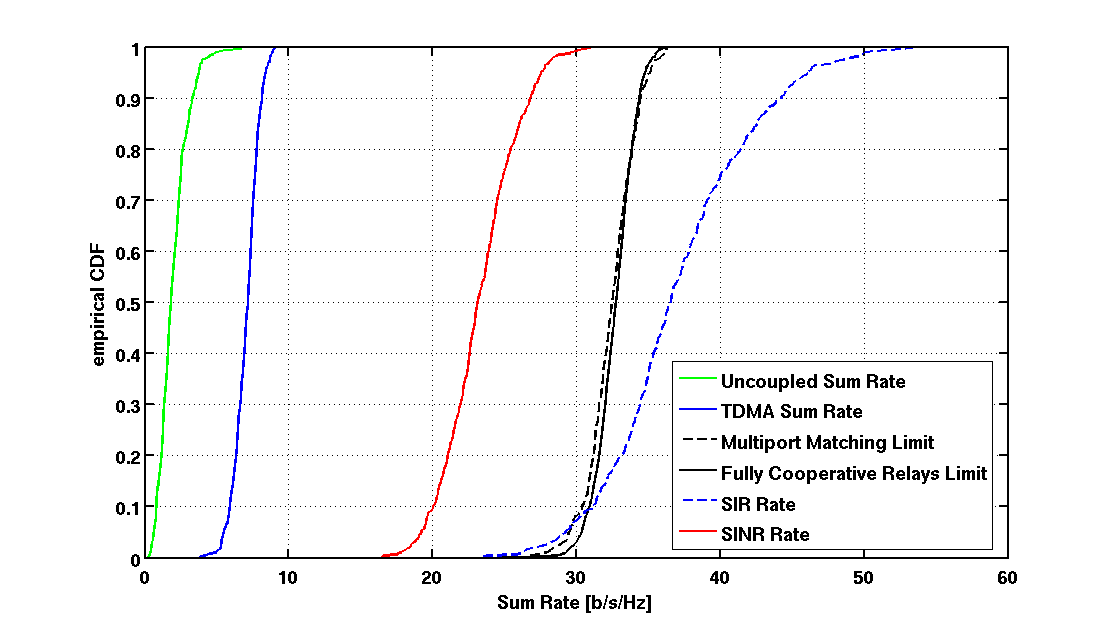
\includegraphics[width=\linewidth]{images/4user_sumrate.png}
\caption{Sum rates of a 4 user MIMO system.}
\label{fig:4user_sumrate}
\end{figure}

Figure~\ref{fig:4user_sumrate} shows the sum rate of the optimized system (red solid curve) compared to the rates we introduced in the beginning of this chapter.
We see that the uncoupled rate~---~in which each receiver has only one receiver antenna and no relays~---~and the TDMA rate (under the sum power constraint) are outperformed by far.
Further, we see that the noise-free rate (dashed blue line) is always larger by at least  $10 \left[\text{b/s/Hz}\right]$, which lets us assume, that the interference cancellation was performed well and that we are in an interference-free region for at least some users.
The black curves denoting the fully cooperative relays limit and the multi-port matching limit (dashed curve) are between $5 \left[\text{b/s/Hz}\right]$ and $10 \left[\text{b/s/Hz}\right]$ bits per second larger than the optimized sum rate.
From Figure~\ref{fig:relcomp_3} we know that the limits are around $2 \left[\text{b/s/Hz}\right]$ larger than the optimized sum rate per user.
This shows that, at the median for four users, the optimization algorithm performs almost as well as for one user, however the lower rates seem to suffer from poor optimization.

\begin{figure}[h]
\centering
  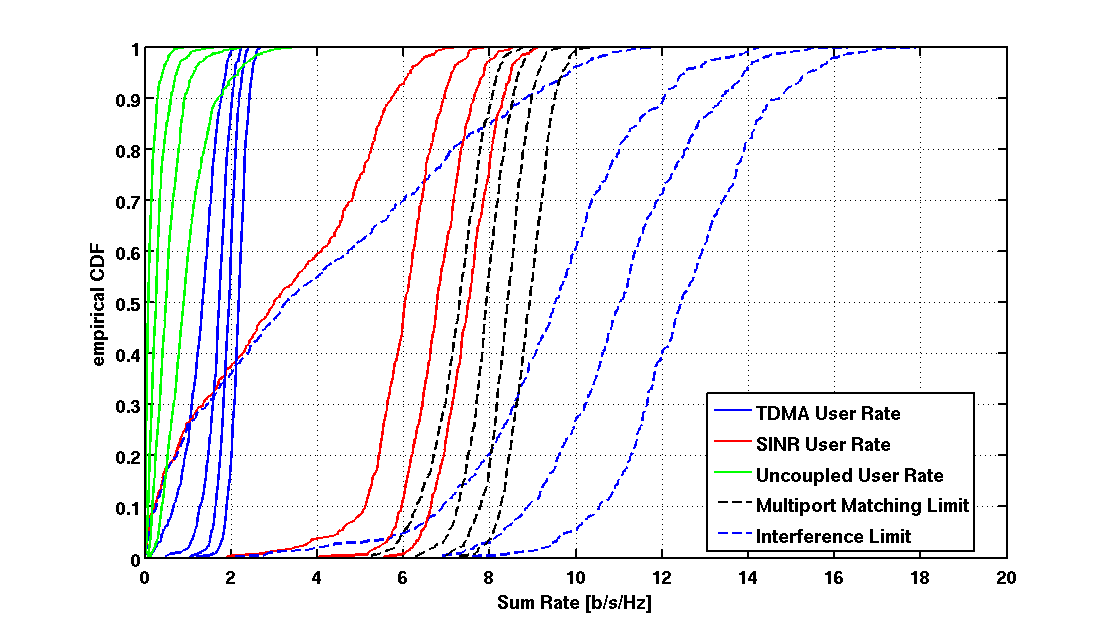
\includegraphics[width=\linewidth]{images/4user_userrate.png}
\caption{The user rates for  four users with seven relays each.}
\label{fig:4user_userrate}
\end{figure}
We saw in Figure~\ref{fig:relcomp_3} that it requires at least seven relays for one user to eliminate the interference from three users.
Figure~\ref{fig:4user_userrate} shows the rates for each transmit/receive pair in red solid curves.
Again, the black dashed curves denote multi-port matching rates, the green solid lines denote performance if the relays are uncoupled, and the blue solid line shows the TDMA rate for each user under the sum power constraint.


We observe that the uncoupled rate as well as the TDMA rate are outperformed by around $5 \left[\text{b/s/Hz}\right]$ for the three top users at the median.
The lowest user, however, is~---~contradicting to the results from Section~\ref{sec:3interf}~---~not interference-free for almost 50\% of cases.
For 10\% of cases, it even shows worse performance than the TDMA rate.
It seems, that this user is, for some realizations, blocked in order to enhance the other three users.
This might be the optimal solution, but it might also be that the solver did not reach the best optimum.

To explore this a little bit further, Figure~\ref{fig:4user_placing} shows typical placings when the minimum user rate could be improved strongly (on the left) and when the rate could only be improved a little (on the right).
Both subplots show a field of size $2\lambda \times 2\lambda$.
For the left subplot, the receivers have larger distances between them and the relays' belonging to the receivers can be easy distinguished~---~they are more or less nicely separated.
This also accounts for receivers one and three in the subplot on the right, but here receivers two and four are not so nicely separated.
Additionally their distance is smaller than $0.5\lambda$.
This leads to stronger coupling between the receiving elements of receivers two and four.
\begin{figure}[h]
\centering
  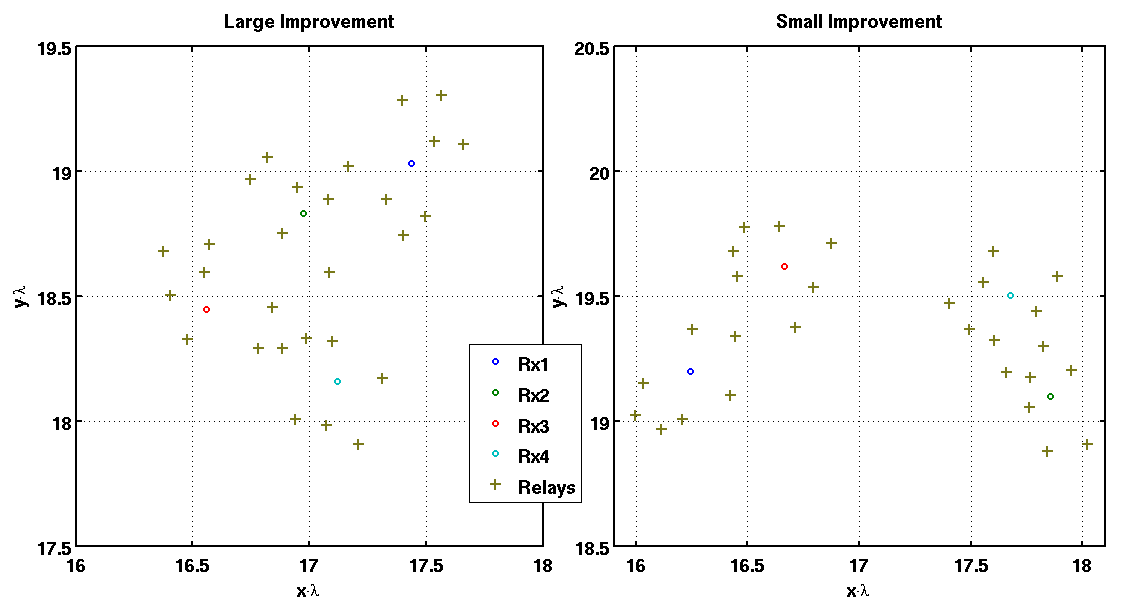
\includegraphics[width=0.8\linewidth]{images/Antenna_placing_4user.png}
\caption{Two different antenna placings, the left leads to a big improvement; the right to a small improvement.}
\label{fig:4user_placing}
\end{figure}
For the optimization, this means that if one receiver and its relays are optimized their coupling might diminish the rate of the other receiver severely.
This effect can be seen as an additional interferer.
Any poor channel realization can lead to a case in which the second receiver rate cannot be optimized significantly.


\section{TDMA - Combination}
\label{sec:tdma_combination}
We assess the combination of our optimization method with currently existing interference-avoiding methods.
As seen in the previous sections, the number of required relays for reducing interference grows with the number of users in the the system.
For large systems with hundreds of users, the required number of relays would become extremely large, hence the optimization very complex.
Therefore, a combination of our strategy with the TDMA method is one way to reduce the number of users in a single time slot, therefore reducing the number of required relays.
\begin{figure}[h]
\centering
  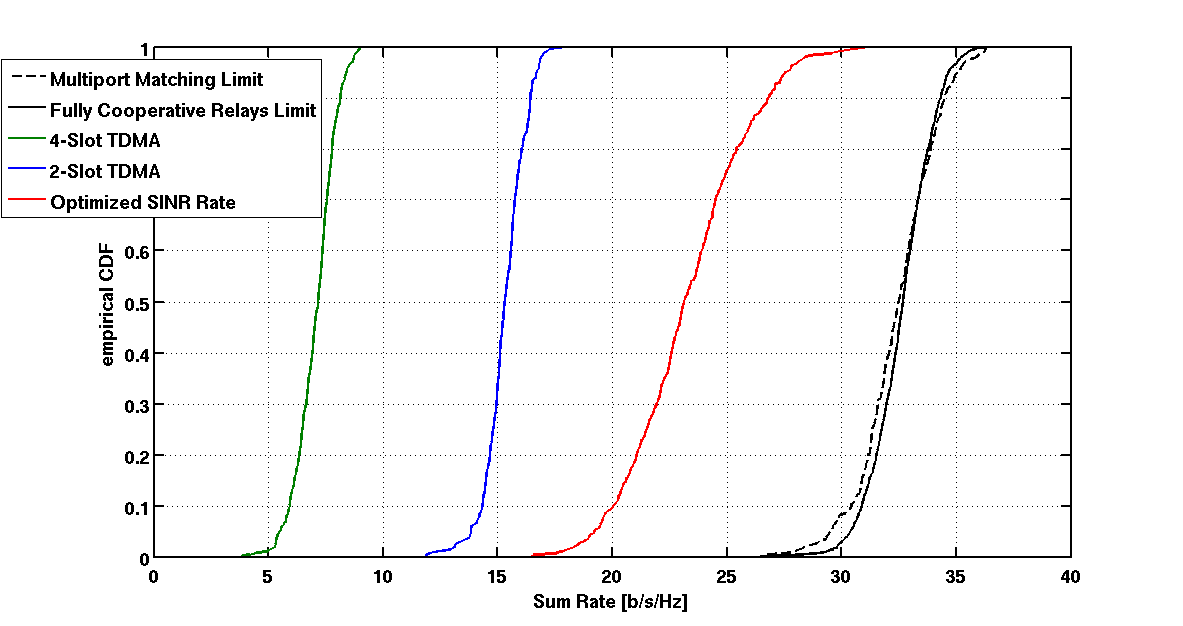
\includegraphics[width=0.9\linewidth]{images/SlotTDMAcomparison_edited.png}
\caption{Comparison of different slot TDMA approaches.}
\label{fig:tdma_comb}
\end{figure}

Using two-slot TDMA, reduces the number of users per slot from four to two.
Therefore, the results from Figure~\ref{fig:4user_sumrate} can be used to compare them to TDMA applied on the results from Figure~\ref{fig:iniopt_comp}.
The combination of TDMA and the optimization introduced in this thesis lead additionally to halving the problem size, therefore yielding results closer to the (corresponding) optimum from 2-slot TDMA than from the pure optimization.
\begin{figure}[h]
\centering
  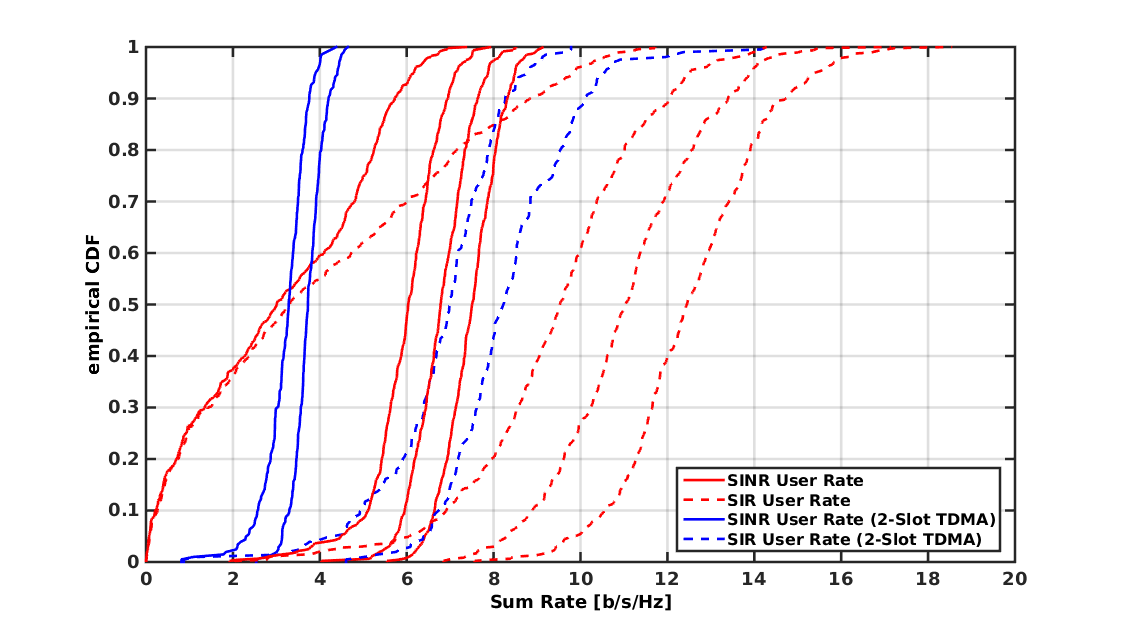
\includegraphics[width=0.9\linewidth]{images/SlotTDMAcomparison_user.png}
\caption{Comparison of different slot TDMA approaches for user rates.}
\label{fig:tdma_comb_user}
\end{figure}

Figure~\ref{fig:tdma_comb} shows in red the results of the four-user system without TDMA (or 1-slot TDMA).
In blue, we show the performance of the 2-slot TDMA approach applied on a four-user system with only three relays per receiver and under the user-power constraint.
In green is the performance of a 4-slot TDMA approach without the use of any relays under the sum-power constraint.
The method introduced in this thesis without the use of TDMA still outperforms 2- and 4-slot TDMA.
However, it can also be observed that the use of only three relays per user and a 2-slot TDMA approach outperforms the pure TDMA approach by approximately $8 \left[\text{b/s/Hz}\right]$.
Hence the combination of using passive relays and TDMA also significantly improves the performance of a system suffering from strong interference.


In Figure~\ref{fig:tdma_comb_user}, we see the user rates for different TDMA approaches.
In blue we see the 2-slot TDMA approach with its SINR- (solid curves) and SIR-rates (dashed curves).
Although the achievable sum rate of the 2-slot TDMA approach is lower than the achievable sum rate of our introduced optimization strategy, it can be seen, that no user experiences blocking in order to improve the sum rate.
Therefore the combination with TDMA is also a method to prevent blocking of users.



